Se mandó a fabricar los chips diseñados para los procesos ONC5 y GF130, en la figura \ref{fig:chip_completo} se muestra los chips con un microscopio electrónico.

\begin{figure}[H]
\subfloat[Chip proceso ONC5]{\label{fig:chip_onc5}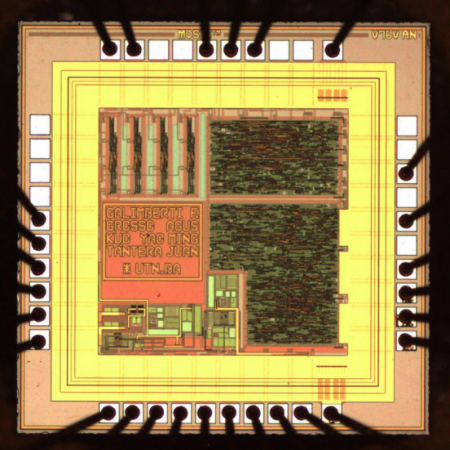
\includegraphics[width=0.5\linewidth]{chip_500.png}}
\subfloat[Chip proceso GF130]{\label{fig:chip_gf130}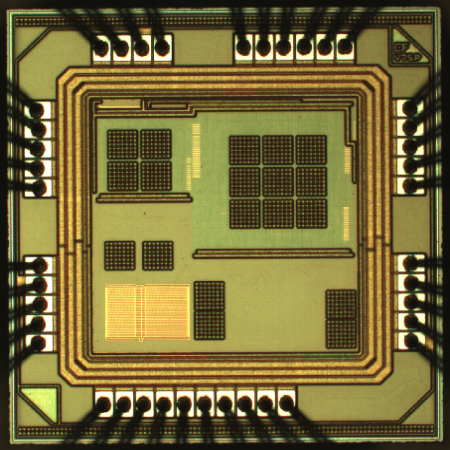
\includegraphics[width=0.5\linewidth]{chip_130.png}}
\caption{Layout del Front-End Analógico}
\label{fig:chip_completo}
\end{figure}

Para validar y verificar los diseños, todos los módulos son testeados y comparados con resultados de simulación. La antena es de 40 x 40 mm, de 4 vueltas, y están hechos sobra un PCB de 35 um de espesor de cobre. 

En la figura \ref{fig:banco} se muestra el banco de medición. Se usó el \textit{NFC shield Adafruit PN532} que actúa como PCD, fuentes de tensión continua para alimentar a los pads de los integrados, un osciloscopio y un analizador lógico Agilent 16806A para validar el protocolo digital. 

Se validó con dos maquinas de estados que cumplen la misma función: 

\begin{itemize}
	\item Banco de pruebas con una FPGA. 
	\item NFC core de Ramiro Gonzalez del Cerro fabricado en el proceso GF130 (Global Foundries 130 nm 8RF).
	\item NFC core de Leandro Tozzi \cite{lascas_std} con las 100 celdas estándar caracterizadas y validadas para el proceso ONC5 (On Semiconductor 500 nm).
\end{itemize}
 

\begin{figure}[H]
\centering
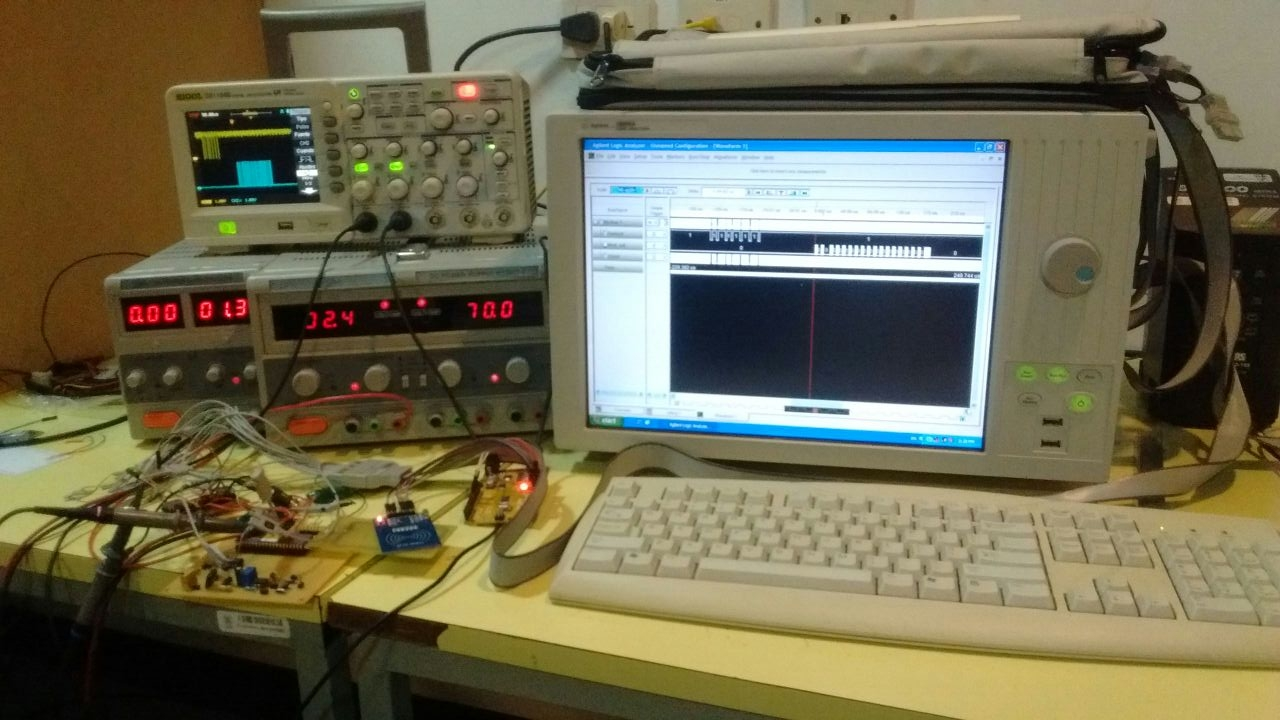
\includegraphics[width=0.8\linewidth]{mediciones/banco.jpeg}
\caption{Banco de medición}
\label{fig:banco}
\end{figure}

Se procedió a medir con el osciloscopio el correcto funcionamiento de los módulos analógicos. En la figura \ref{fig:med_clk_demod} se muestra el clock 13.56/4 MHz (canal 1) y la modulación PCD a PICC (canal 2). Como podemos observar, el clock se apaga cuando viene una modulación desde el lector.

En la figura \ref{fig:power_on_reset} se puede observar el funcionamiento del módulo Power on Reset (canal 2). Cuando se energiza el chip (canal 1), el módulo POR tarda algunos milisegundos en poner en 1 lógico, ésto nos permite resetear el core digital.

\begin{figure}[H]
\subfloat[Clock vs Demodulación]{\label{fig:med_clk_demod}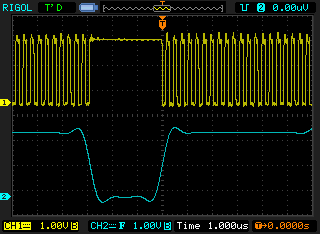
\includegraphics[width=0.5\linewidth]{mediciones/demod.png}}
\subfloat[Power on Reset]{\label{fig:power_on_reset}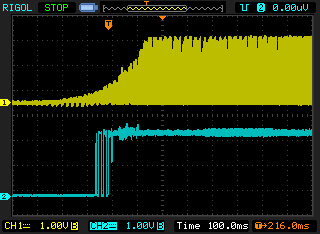
\includegraphics[width=0.5\linewidth]{mediciones/por.png}}
\caption{Mediciones del Front-End Analógico}

\label{fig:med_afe}
\end{figure}

Para validar el AFE, se envió uno de los primeros comandos definidos en la norma ISO/IEC 14443 \ref{sec:iso}. Se observa en las figuras \ref{fig:digital_nfc} y \ref{fig:digital_nfc2} que los chips responden correctamente al comando REQA enviado desde la PCD contestando el comando ATQA.


\begin{figure}[H]
\centering
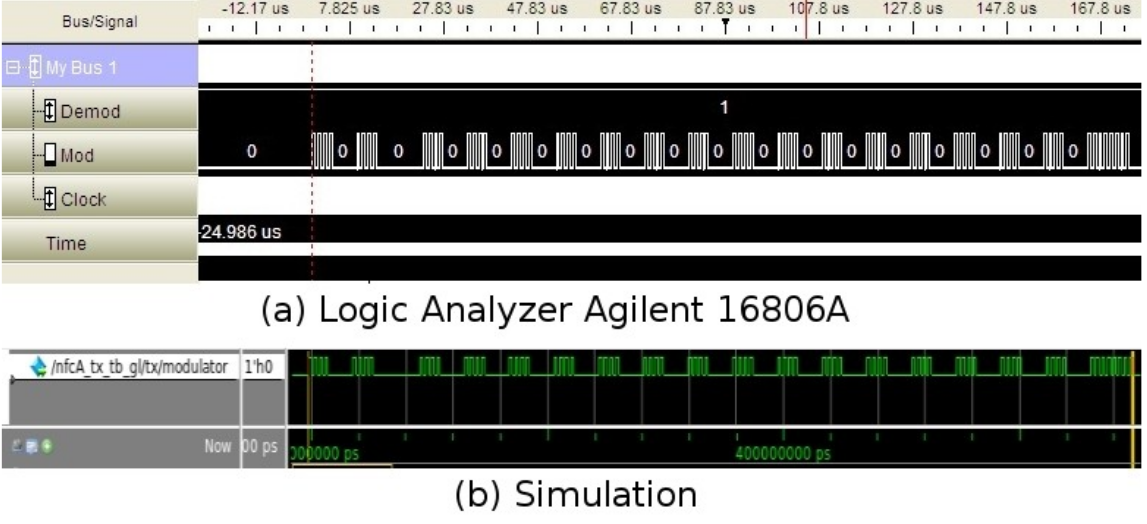
\includegraphics[width=0.8\linewidth]{mediciones/nfc.png}
\caption{Mediciones del core NFC}
\label{fig:digital_nfc}
\end{figure}

\begin{figure}[H]
\centering
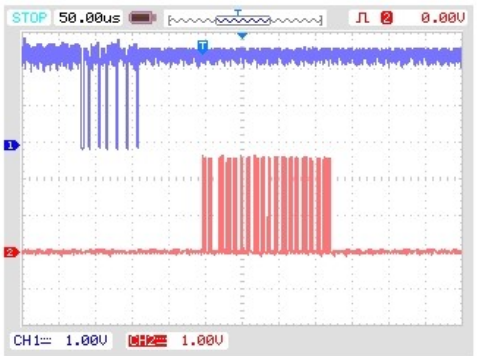
\includegraphics[width=0.3\linewidth]{mediciones/nfc2.png}
\caption{Respuesta al comando REQA}
\label{fig:digital_nfc2}
\end{figure}